% 第6章 常规态型近场动力学
\chapter{常规态型近场动力学}

\leavevmode\usetikzlibrary{arrows.meta}

\section{态型理论的基本概念与数学表述}

第 4 章与第 5 章介绍的键型理论以对力函数为唯一的本构工具，其运动方程形式简洁、数值实现方便，在断裂模拟中获得了广泛应用。然而，对力函数仅依赖单根键的变形这一基本假设，使键型理论在描述一般工程材料时遭遇了根本困难。本节首先剖析键型理论的本质局限，引出态（state）这一核心概念（\ref{sec:state-limits}节），进而给出变形态与力态的严格定义及其代数运算（\ref{sec:state-defs}节），在此基础上建立态型运动方程（\ref{sec:state-motion}节），并据力态与变形后键方向的关系将态型理论划分为常规态型与非常规态型两类（\ref{sec:osb-nosb}节），最后引入弹性态、简单材料与膨胀等本构基本概念（\ref{sec:elastic-states}节），为\ref{sec:osb-elastic}节常规态型弹性本构模型的建立奠定基础。本节内容全部源自 Silling 等提出的态型理论原始文献 \cite{Silling2007}，守恒律的公理化处理与严格证明见第 2 章及文献 \cite{SillingLehoucq2010}。

\subsection{键型理论的局限与态的引入}\label{sec:state-limits}

键型理论的一切局限，都可以追溯到对力函数仅依赖单根键的变形这一基本假设。回顾第 4 章，键型理论中材料点 $\mathbf{x}$ 所受合力为对力密度 $\mathbf{f}(\boldsymbol{\eta},\boldsymbol{\xi})$ 在其近场域 $H_{\mathbf{x}}$ 上的积分，而 $\mathbf{f}$ 的自变量只有该键的相对位移 $\boldsymbol{\eta}=\mathbf{u}(\mathbf{x}',t)-\mathbf{u}(\mathbf{x},t)$ 与参考方向矢量 $\boldsymbol{\xi}=\mathbf{x}'-\mathbf{x}$，即键的力完全由该键自身的伸长决定，与近场域内其他键的变形无关。线动量守恒要求对力函数满足反对称条件 $\mathbf{f}(-\boldsymbol{\eta},-\boldsymbol{\xi})=-\mathbf{f}(\boldsymbol{\eta},\boldsymbol{\xi})$，即在成对相互作用的意义上满足牛顿第三定律 \cite{Silling2000}。对于微弹性（microelastic）材料，对力可由成对势函数（pairwise potential）$w(\boldsymbol{\eta},\boldsymbol{\xi})$ 导出，应变能密度取成对势之和的形式
\[
  W=\frac{1}{2}\int_{H_{\mathbf{x}}}w(\boldsymbol{\eta},\boldsymbol{\xi})\,dV_{\mathbf{x}'}
\]
其中系数 $1/2$ 源于每一对键的势能被两个端点各计入一次 \cite{Silling2000,Silling2007}。这种中心对称的成对势结构意味着，材料点层面的相互作用只有一个沿键方向的“轴向”通道，不存在与方向相关的独立剪切通道。

成对势结构直接导致两个后果。其一，对三维各向同性材料而言，可标定的弹性常数只有一个，体积模量与剪切模量不能独立取值，泊松比被迫固定为 $1/4$；对二维平面应力问题，泊松比固定为 $1/3$ \cite{SillingAskari2005,Silling2007}。而工程材料的泊松比通常在 $1/4$ 之上（如钢约为 $0.3$，橡胶接近 $0.5$），键型理论无法描述这类材料。其二，也是更本质的，键型理论无法刻画体积变形与剪切变形的独立响应：键的伸长同时包含体积变化与形状变化的贡献，单个伸长量无法将二者区分，因此任何基于单键伸长的本构都无法独立调节材料对体积变形与剪切变形的抵抗力 \cite{Silling2007}。第 5 章介绍的微梁模型、共轭键模型等改进方案，正是试图在键的层次引入额外的弯曲、扭转自由度来部分缓解这一困难，但这些方案本质上仍在成对相互作用的框架内修补，未能从根本上解除限制。

突破这一局限的关键，在于放弃“材料点的力学响应由单根键的变形决定”这一前提，转而承认材料点感受的是整个近场域内的变形构型。Silling 等 2007 年提出的态型（state-based，第 1 章亦称态基）理论正是沿着这一思路对近场动力学基本方程的重新表述 \cite{Silling2007}。该理论的核心思想是：把材料点近场域内全部键的变形信息组织为一个称为态（state）的数学对象，材料点的受力由这个态通过本构关系确定。图\ref{fig:state-map}示意了态的概念：材料点 $\mathbf{x}$ 的变形态对近场域内每一根键赋予一个矢量值，这些值共同构成 $\mathbf{x}$ 处变形状态的完整描述；与之相比，键型理论中的对力函数只是这个态在单根键上的一个函数值。

\begin{figure}[htbp]
  \centering
  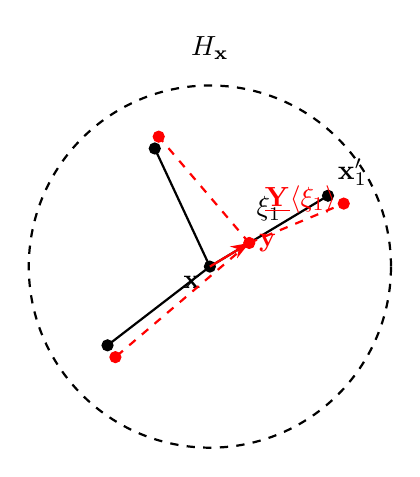
\begin{tikzpicture}[scale=1.0]
    % 近场域
    \draw[dashed, thick] (0,0) circle (2.3);
    \node[above] at (0,2.5) {$H_{\mathbf{x}}$};
    % 参考构型：中心点与三个邻点
    \filldraw (0,0) circle (2pt) node[below left] {$\mathbf{x}$};
    \draw[thick] (0,0) -- (1.5,0.9);
    \draw[thick] (0,0) -- (-0.7,1.5);
    \draw[thick] (0,0) -- (-1.3,-1.0);
    \filldraw (1.5,0.9) circle (2pt);
    \filldraw (-0.7,1.5) circle (2pt);
    \filldraw (-1.3,-1.0) circle (2pt);
    \node[above right] at (1.5,0.9) {$\mathbf{x}'_1$};
    % 变形后构型
    \filldraw[red] (0.5,0.3) circle (2pt);
    \node[red, right] at (0.5,0.3) {$\mathbf{y}$};
    \draw[-Stealth, thick, red] (0,0) -- (0.5,0.3);
    \draw[dashed, thick, red] (0.5,0.3) -- (1.7,0.8);
    \draw[dashed, thick, red] (0.5,0.3) -- (-0.65,1.65);
    \draw[dashed, thick, red] (0.5,0.3) -- (-1.2,-1.15);
    \filldraw[red] (1.7,0.8) circle (2pt);
    \filldraw[red] (-0.65,1.65) circle (2pt);
    \filldraw[red] (-1.2,-1.15) circle (2pt);
    % 标注
    \node[above] at (0.75,0.45) {$\boldsymbol{\xi}_1$};
    \node[red, above] at (1.15,0.55) {$\underline{\mathbf{Y}}\langle\boldsymbol{\xi}_1\rangle$};
  \end{tikzpicture}
  \caption{态的概念示意，变形态将近场域内每一根键映射为其变形后矢量，完整描述材料点处的变形构型}
  \label{fig:state-map}
\end{figure}

\subsection{态的定义与代数运算}\label{sec:state-defs}

要严格定义态，首先需要固定记号。材料点 $\mathbf{x}$ 在时刻 $t$ 的变形后位置记为
\[
  \mathbf{y}(\mathbf{x},t)=\mathbf{x}+\mathbf{u}(\mathbf{x},t)
\]
其中 $\mathbf{u}$ 为位移场。连接 $\mathbf{x}$ 与 $\mathbf{x}'$ 的键矢量仍记为 $\boldsymbol{\xi}=\mathbf{x}'-\mathbf{x}$，变形后该键两端点的相对位置变为 $\mathbf{y}(\mathbf{x}',t)-\mathbf{y}(\mathbf{x},t)$。在此基础上给出变形态的定义。

\begin{definition}
  材料点 $\mathbf{x}$ 在时刻 $t$ 的变形态（deformation state）$\underline{\mathbf{Y}}[\mathbf{x},t]$ 是定义在近场域 $H_{\mathbf{x}}$ 内所有键矢量上的映射，其值为
  \begin{equation}
    \underline{\mathbf{Y}}[\mathbf{x},t]\langle\boldsymbol{\xi}\rangle=\boldsymbol{\xi}+\boldsymbol{\eta}=\mathbf{y}(\mathbf{x}',t)-\mathbf{y}(\mathbf{x},t)
    \label{eq:deformation-state}
  \end{equation}
  其中 $\boldsymbol{\eta}=\mathbf{u}(\mathbf{x}',t)-\mathbf{u}(\mathbf{x},t)$ 为相对位移。
\end{definition}

式\eqref{eq:deformation-state}中，$\underline{\mathbf{Y}}[\mathbf{x},t]\langle\boldsymbol{\xi}\rangle$ 表示变形态作用于键矢量 $\boldsymbol{\xi}$ 所得的值，即该键变形后的矢量。这里采用了态理论的三重符号约定：下划线表示态，方括号内是态的定义参数（材料点与时刻），尖括号 $\langle\cdot\rangle$ 表示态对其自变量——键矢量的求值。变形态把近场域内的每一根键映射为其变形后矢量，因而完整刻画了 $\mathbf{x}$ 处近场域内的变形构型。态与经典场量的根本区别在于：经典场量（如应力张量）以材料点的位置为自变量，取值于该点；态则以相对矢量（键）为自变量，把一族键整体映射为一系列值，因此态是定义在“以 $\mathbf{x}$ 为中心的一束键”上的对象，天然携带了非局部信息 \cite{Silling2007}。

与变形态对应，力态（force state）$\underline{\mathbf{T}}[\mathbf{x},t]$ 同样是键矢量到矢量的映射，$\underline{\mathbf{T}}[\mathbf{x},t]\langle\boldsymbol{\xi}\rangle$ 表示 $\mathbf{x}$ 处力态在键 $\boldsymbol{\xi}$ 上的力密度取值，其量纲与键型理论中的对力密度相同（三维情形为 $\mathrm{N/m^6}$）。材料点沿键获得的净力密度由两个端点的力态之差给出，具体见 \ref{sec:state-motion}节。

态按其值的类型可分为标量态与矢量态两类，此外还可通过张量积得到张量值态。变形态与力态都是矢量态。标量态最典型的例子是伸长态（extension state）$\underline{e}$，定义为
\begin{equation}
  \underline{e}[\mathbf{x},t]\langle\boldsymbol{\xi}\rangle=\bigl|\underline{\mathbf{Y}}[\mathbf{x},t]\langle\boldsymbol{\xi}\rangle\bigr|-|\boldsymbol{\xi}|
  \label{eq:extension-state}
\end{equation}
即变形后键长与参考键长之差。伸长态与键型理论中的伸长率直接对应，关系为 $s=\underline{e}\langle\boldsymbol{\xi}\rangle/|\boldsymbol{\xi}|$ \cite{Silling2007}。态型理论中还会用到其他标量态，如刻画局部体密度分布的加权体密度态（weighted body density state）\cite{Silling2010,SillingLehoucq2010}，以及\ref{sec:elastic-states}节将引入的权重函数等。

态的定义域与值域确定之后，还需要规定态与态之间的代数运算，才能把多个态组合成本构表达式。设 $\underline{\mathbf{A}}$、$\underline{\mathbf{B}}$ 为定义在同一近场域上的态，$\alpha$ 为标量，态的加法与数乘逐键定义为
\[
  (\underline{\mathbf{A}}+\underline{\mathbf{B}})\langle\boldsymbol{\xi}\rangle=\underline{\mathbf{A}}\langle\boldsymbol{\xi}\rangle+\underline{\mathbf{B}}\langle\boldsymbol{\xi}\rangle,\qquad
  (\alpha\,\underline{\mathbf{A}})\langle\boldsymbol{\xi}\rangle=\alpha\,\underline{\mathbf{A}}\langle\boldsymbol{\xi}\rangle
\]
在此运算下，所有定义域相同、值域相同的态构成一个线性空间。态的点积（dot product）定义为
\begin{equation}
  \underline{\mathbf{A}}\cdot\underline{\mathbf{B}}=\int_{H_{\mathbf{x}}}\underline{\mathbf{A}}\langle\boldsymbol{\xi}\rangle\cdot\underline{\mathbf{B}}\langle\boldsymbol{\xi}\rangle\,dV_{\mathbf{x}'}
  \label{eq:state-dot-product}
\end{equation}
对两个矢量态，上式给出一个标量；对两个标量态，被积函数改为对应标量值的乘积，结果同样为标量。态的点积为应变能等积分型表达式提供了紧凑的记号（见 \ref{sec:elastic-states}节）。态的张量积（dyadic product）定义为
\[
  (\underline{\mathbf{A}}\otimes\underline{\mathbf{B}})\langle\boldsymbol{\xi}\rangle=\underline{\mathbf{A}}\langle\boldsymbol{\xi}\rangle\otimes\underline{\mathbf{B}}\langle\boldsymbol{\xi}\rangle
\]
其值为二阶张量，可用于构造形状张量等二阶量（第 7 章）。此外还常用到两类特殊态：单位态（identity state）$\underline{\mathbf{I}}$ 与标量单位态 $\underline{1}$，满足 $\underline{\mathbf{I}}\langle\boldsymbol{\xi}\rangle=\boldsymbol{\xi}$、$\underline{1}\langle\boldsymbol{\xi}\rangle=1$；零态（zero state）$\underline{\mathbf{0}}$ 满足 $\underline{\mathbf{0}}\langle\boldsymbol{\xi}\rangle=\mathbf{0}$。借助这些记号，伸长态可写为 $\underline{e}=|\underline{\mathbf{Y}}|-|\underline{\mathbf{I}}|$，形式更为简洁 \cite{Silling2007,MadenciOterkus2014}。

\begin{remark}
  态与经典张量场的区别值得反复强调。应力张量 $\boldsymbol{\sigma}(\mathbf{x})$ 在点 $\mathbf{x}$ 处取值，是局部对象；而态 $\underline{\mathbf{T}}[\mathbf{x},t]$ 是对一族键取值的映射，是整体对象。态理论之所以能解除键型理论的成对性限制，根源正在于本构关系可以同时“看见”近场域内的全部键，而这一点在经典的场量表述中是无法实现的。
\end{remark}

\subsection{态型运动方程}\label{sec:state-motion}

态型理论中，运动方程以力态的“差”取代键型理论中的对力函数。材料点 $\mathbf{x}$ 的运动方程为
\begin{equation}
  \rho(\mathbf{x})\ddot{\mathbf{u}}(\mathbf{x},t)=\int_{H_{\mathbf{x}}}\Bigl(\underline{\mathbf{T}}[\mathbf{x},t]\langle\boldsymbol{\xi}\rangle-\underline{\mathbf{T}}[\mathbf{x}',t]\langle-\boldsymbol{\xi}\rangle\Bigr)dV_{\mathbf{x}'}+\mathbf{b}(\mathbf{x},t)
  \label{eq:state-motion}
\end{equation}
其中 $\rho$ 为质量密度，$\mathbf{b}$ 为体力密度。为书写简洁，将 $\mathbf{x}'$ 处的力态记为 $\underline{\mathbf{T}}'=\underline{\mathbf{T}}[\mathbf{x}',t]$。被积函数中第一项 $\underline{\mathbf{T}}\langle\boldsymbol{\xi}\rangle$ 是 $\mathbf{x}$ 处力态在键 $\boldsymbol{\xi}$ 上的取值，第二项 $\underline{\mathbf{T}}'\langle-\boldsymbol{\xi}\rangle$ 是 $\mathbf{x}'$ 处力态在反向键 $-\boldsymbol{\xi}$ 上的取值；二者之差 $\underline{\mathbf{T}}\langle\boldsymbol{\xi}\rangle-\underline{\mathbf{T}}'\langle-\boldsymbol{\xi}\rangle$ 即为 $\mathbf{x}$ 沿该键获得的净力密度。注意 $\underline{\mathbf{T}}'$ 的自变量必须是 $-\boldsymbol{\xi}=\mathbf{x}-\mathbf{x}'$，因为从 $\mathbf{x}'$ 出发指向 $\mathbf{x}$ 的键矢量正是 $-\boldsymbol{\xi}$。

与键型运动方程对比，式\eqref{eq:state-motion}的结构来源一目了然：键型理论把“$\mathbf{x}$ 对 $\mathbf{x}'$ 的作用”与“$\mathbf{x}'$ 对 $\mathbf{x}$ 的作用”合并为一个成对函数 $\mathbf{f}$，并要求二者大小相等、方向相反；态型理论则把这两个作用分开表述，各自由作用点处的力态给出，成对性不再是先验的假设。事实上，当力态取特殊形式
\[
  \underline{\mathbf{T}}\langle\boldsymbol{\xi}\rangle=\frac{1}{2}\mathbf{f}(\boldsymbol{\eta},\boldsymbol{\xi})
\]
时，由反对称条件 $\mathbf{f}(-\boldsymbol{\eta},-\boldsymbol{\xi})=-\mathbf{f}(\boldsymbol{\eta},\boldsymbol{\xi})$ 可得
\[
  \underline{\mathbf{T}}'\langle-\boldsymbol{\xi}\rangle=\frac{1}{2}\mathbf{f}(-\boldsymbol{\eta},-\boldsymbol{\xi})=-\frac{1}{2}\mathbf{f}(\boldsymbol{\eta},\boldsymbol{\xi})
\]
代入式\eqref{eq:state-motion}后即回到键型运动方程。可见键型理论是态型理论在成对性约束下的特例，态型运动方程在形式上包含了键型运动方程 \cite{Silling2007}。

式\eqref{eq:state-motion}的守恒性质值得说明。无外载荷时，将式\eqref{eq:state-motion}对全物体 $\mathcal{B}$（物体所占区域）积分，并交换积分变量 $\mathbf{x}\leftrightarrow\mathbf{x}'$，可知双重积分中两项
\[
  \int_{\mathcal{B}}\int_{H_{\mathbf{x}}}\underline{\mathbf{T}}[\mathbf{x},t]\langle\boldsymbol{\xi}\rangle\,dV_{\mathbf{x}'}\,dV
  \quad\text{与}\quad
  \int_{\mathcal{B}}\int_{H_{\mathbf{x}}}\underline{\mathbf{T}}[\mathbf{x}',t]\langle-\boldsymbol{\xi}\rangle\,dV_{\mathbf{x}'}\,dV
\]
完全相等而相消，故 $\int_{\mathcal{B}}\rho\ddot{\mathbf{u}}\,dV=\mathbf{0}$，即线动量对任意力态自动守恒 \cite{Silling2007}。角动量守恒则不自动成立，需要更强的条件，例如对弹性材料，应变能密度须具有旋转不变性。这些条件的严格表述与证明将在第 2 章给出 \cite{SillingLehoucq2010}。式\eqref{eq:state-motion}是态型理论的核心方程，也是全书的中心方程之一：\ref{sec:osb-elastic}节起建立的各类态型本构模型都以它为运动框架，只需给定力态 $\underline{\mathbf{T}}$ 的具体形式即可封闭方程组。

\subsection{常规态型与非常规态型}\label{sec:osb-nosb}

力态与变形后键方向的关系，是划分态型理论类型的首要判据。若力态 $\underline{\mathbf{T}}\langle\boldsymbol{\xi}\rangle$ 与变形态 $\underline{\mathbf{Y}}\langle\boldsymbol{\xi}\rangle$ 共线，即力的方向恒沿变形后键的方向，则称为常规态型（ordinary state-based，OSB）。此时力态可以写成
\begin{equation}
  \underline{\mathbf{T}}\langle\boldsymbol{\xi}\rangle=\underline{t}\langle\boldsymbol{\xi}\rangle\,\underline{\mathbf{M}}\langle\boldsymbol{\xi}\rangle
  \label{eq:osb-force}
\end{equation}
其中
\[
  \underline{\mathbf{M}}\langle\boldsymbol{\xi}\rangle=\frac{\underline{\mathbf{Y}}\langle\boldsymbol{\xi}\rangle}{\bigl|\underline{\mathbf{Y}}\langle\boldsymbol{\xi}\rangle\bigr|}
\]
为单位方向态（direction state），指向变形后键的方向；$\underline{t}$ 为标量力态（scalar force state），它是标量态，其值可以依赖材料点近场域内的整个变形构型 \cite{Silling2007}。

式\eqref{eq:osb-force}的意义在于：OSB 保留了“力沿键方向”这一键型特征，因而断键准则、损伤描述等基于键方向的概念可以延续使用；但 $\underline{t}$ 的取值不再受成对势约束，可以随族内其他键的变形而变，因此体积模量与剪切模量可以独立标定，泊松比限制被彻底解除。事实上，当取 $\underline{t}=cs/2$（其中 $c$ 为微模量，$s$ 为伸长率）时，式\eqref{eq:osb-force}回到键型 PMB 模型的力态表述，再次印证了键型理论是态型理论的特例 \cite{Silling2007}。本章后续各节（\ref{sec:osb-elastic}节弹性本构、\ref{sec:osb-plastic}节弹塑性、\ref{sec:strength-params}节强度参数）讨论的都是常规态型理论。

若力态不要求与变形后键方向共线，即允许键上传递偏离键方向的力，则称为非常规态型（non-ordinary state-based，NOSB）。非常规态型可以描述键上的剪切与转动传递，其典型实现是本构对应（constitutive correspondence）机制：通过非局部变形梯度构造近似经典应力张量，把经典连续介质力学的本构模型直接嵌入态型框架，此时力态的方向与大小都由经典应力张量决定，一般不再沿键方向 \cite{Silling2007,Javili2019}。本构对应机制及其数值实现将在第 7 章详细讨论。图\ref{fig:osb-nosb}对比了两类态型的力方向特征：常规态型的力恒沿变形后键方向，非常规态型的力可以偏离键方向。

\begin{figure}[htbp]
  \centering
  \begin{tikzpicture}[scale=1.0]
    % (a) OSB
    \filldraw (0,0) circle (2pt) node[below] {$\mathbf{x}$};
    \filldraw (2.2,1.2) circle (2pt) node[above right] {$\mathbf{y}'$};
    \draw[thick] (0,0) -- (2.2,1.2);
    \draw[-Stealth, thick, red] (0,0) -- (1.0,0.55);
    \node[red, above] at (0.55,0.3) {$\underline{\mathbf{T}}=\underline{t}\,\underline{\mathbf{M}}$};
    \node[below] at (1.1,-0.35) {(a) 常规态型};
    % (b) NOSB
    \begin{scope}[xshift=5.4cm]
      \filldraw (0,0) circle (2pt) node[below] {$\mathbf{x}$};
      \filldraw (2.2,1.2) circle (2pt) node[above right] {$\mathbf{y}'$};
      \draw[thick] (0,0) -- (2.2,1.2);
      \draw[dashed, gray] (0,0) -- (1.056,0.576);
      \draw[-Stealth, thick, red] (0,0) -- (0.53,1.08);
      \node[red, above] at (0.2,1.15) {$\underline{\mathbf{T}}$};
      \node[below] at (1.1,-0.35) {(b) 非常规态型};
    \end{scope}
  \end{tikzpicture}
  \caption{常规态型与非常规态型力方向对比，OSB 力态与变形后键方向共线，NOSB 力态可偏离键方向}
  \label{fig:osb-nosb}
\end{figure}

两类态型在数学结构与数值性质上也有重要差异。OSB 的力沿键方向，其弹性本构可以由一个标量势函数（应变能密度）导出，结构简单、稳定性好；NOSB 由于引入了类似经典应力张量的中间量，本构表达灵活，但可能产生零能模式（zero-energy mode）等数值失稳问题 \cite{Javili2019}。这些差异将在本章后续节与第 7 章中逐步展开。

\subsection{弹性态与本构概念}\label{sec:elastic-states}

态型框架下的本构理论以弹性态（elastic state）为起点。若存在一个以变形态为自变量的可微标量函数 $W(\underline{\mathbf{Y}})$，称为应变能密度函数，使得力态等于 $W$ 对 $\underline{\mathbf{Y}}$ 的 Fréchet 导数，即对任意变形态增量 $\Delta\underline{\mathbf{Y}}$ 有
\begin{equation}
  W(\underline{\mathbf{Y}}+\Delta\underline{\mathbf{Y}})=W(\underline{\mathbf{Y}})+\underline{\mathbf{T}}\cdot\Delta\underline{\mathbf{Y}}+o\bigl(\|\Delta\underline{\mathbf{Y}}\|\bigr)
  \label{eq:elastic-material}
\end{equation}
则称该材料为弹性材料。式中 $\underline{\mathbf{T}}\cdot\Delta\underline{\mathbf{Y}}$ 为态点积（见式\eqref{eq:state-dot-product}），$\|\cdot\|$ 为由点积诱导的范数。由式\eqref{eq:elastic-material}，力态可以形式地写为
\[
  \underline{\mathbf{T}}=\nabla_{\underline{\mathbf{Y}}}W
\]
即力态是应变能密度对变形态的 Fréchet 导数 \cite{Silling2007}。这个定义与经典超弹性理论中应力 $\boldsymbol{\sigma}=\partial W/\partial\mathbf{F}$ 的关系完全类似，区别仅在于自变量：经典理论的自变量是变形梯度 $\mathbf{F}$，描述无穷小邻域内的线性化变形；态型理论的自变量是变形态 $\underline{\mathbf{Y}}$，描述整个近场域内的变形构型。

若材料的本构响应只依赖当前的变形态 $\underline{\mathbf{Y}}[\mathbf{x},t]$（以及 $\mathbf{x}$、$t$ 的显式依赖），不依赖变形历史与更高阶信息，则称为简单材料（simple material）\cite{Silling2007}。\ref{sec:osb-elastic}节建立的线性弹性本构即属此类；\ref{sec:osb-plastic}节讨论的弹塑性材料将通过内变量的引入把历史依赖纳入本构，可以看作简单材料框架的推广。对于弹性材料，线动量守恒自动满足；角动量守恒则对 $W$ 施加限制，其充分条件为 $W$ 具有旋转不变性（客观性）。这些守恒律条件及其对态型本构的约束将在第 2 章系统讨论 \cite{Silling2007,SillingLehoucq2010}。

为建立具体的 OSB 弹性本构（\ref{sec:osb-elastic}节），还需要两个基本概念：权重函数与膨胀。权重函数（influence function）$\omega(|\boldsymbol{\xi}|)$ 是非负的标量函数，刻画不同距离的键在加权平均中的相对重要性，常取常数 $1$ 或随距离线性衰减的形式 $1-|\boldsymbol{\xi}|/\delta$ \cite{Silling2007}，其选取影响本构的精度与表面修正（第 9、10 章）。借助权重函数可定义加权体积（weighted volume）
\begin{equation}
  m=\int_{H_{\mathbf{x}}}\omega(|\boldsymbol{\xi}|)\,\boldsymbol{\xi}\cdot\boldsymbol{\xi}\,dV_{\mathbf{x}'}
  \label{eq:weighted-volume}
\end{equation}
以及伸长态的加权平均——膨胀（dilatation）
\begin{equation}
  \theta=\frac{3}{m}\int_{H_{\mathbf{x}}}\omega(|\boldsymbol{\xi}|)\,|\boldsymbol{\xi}|\,\underline{e}\langle\boldsymbol{\xi}\rangle\,dV_{\mathbf{x}'}
  \label{eq:dilatation}
\end{equation}
其中 $\underline{e}$ 为式\eqref{eq:extension-state}定义的伸长态 \cite{Silling2007}。膨胀是体积应变的非局部度量：对均匀变形 $\underline{\mathbf{Y}}\langle\boldsymbol{\xi}\rangle=\mathbf{F}\boldsymbol{\xi}$（$\mathbf{F}$ 为常变形梯度），在小变形近似下伸长态满足
\[
  \underline{e}\langle\boldsymbol{\xi}\rangle\approx\frac{\boldsymbol{\xi}\cdot\boldsymbol{\varepsilon}\cdot\boldsymbol{\xi}}{|\boldsymbol{\xi}|}
\]
其中 $\boldsymbol{\varepsilon}$ 为小应变张量；又因权重函数仅依赖 $|\boldsymbol{\xi}|$，积分张量 $\int_{H_{\mathbf{x}}}\omega\,\boldsymbol{\xi}\otimes\boldsymbol{\xi}\,dV_{\mathbf{x}'}$ 是各向同性的，取迹并与式\eqref{eq:weighted-volume}比较可知其等于 $(m/3)\mathbf{I}$，于是
\[
  \theta=\frac{3}{m}\int_{H_{\mathbf{x}}}\omega\,\boldsymbol{\xi}\cdot\boldsymbol{\varepsilon}\cdot\boldsymbol{\xi}\,dV_{\mathbf{x}'}
  =\frac{3}{m}\cdot\frac{m}{3}\,\mathrm{tr}\,\boldsymbol{\varepsilon}
  =\mathrm{tr}\,\boldsymbol{\varepsilon}
\]
即均匀小变形下膨胀恰等于经典体积应变。可见膨胀把近场域内键的伸长信息压缩为一个标量，表征材料点的体积变形状态。式\eqref{eq:dilatation}中的系数 $3/m$ 对应三维情形，二维情形的系数为 $2/m$，将在\ref{sec:osb-elastic}节给出 \cite{MadenciOterkus2014}。

膨胀概念的引入使 OSB 本构可以沿“体积—偏斜”两条通道分别标定：标量力态 $\underline{t}$ 中的膨胀项由体积模量与剪切模量的组合 $3k-5\mu$ 标定，伸长态项由剪切模量 $\mu$ 标定（其中 $k$ 为体积模量，$\mu$ 为剪切模量），从而实现了\ref{sec:state-limits}节指出的体积变形与剪切变形的独立响应。这一本构的具体形式将在\ref{sec:osb-elastic}节给出，其线性化分析可参见 \cite{Silling2010,SillingLehoucq2010}；关于态型理论更为系统的综述性论述见文献 \cite{Bobaru2016}。

本节建立了态型理论的基本概念与数学框架：态的定义与运算提供了描述非局部变形与受力的语言，态型运动方程式\eqref{eq:state-motion}取代键型方程成为核心方程，OSB 与 NOSB 的分类界定了本构模型的构造范围，弹性态、简单材料与膨胀则奠定了本构理论的基础。\ref{sec:osb-elastic}节将在此基础上建立线性各向同性 OSB 弹性本构并推广到复合材料层合板，\ref{sec:osb-plastic}节讨论弹塑性模型，\ref{sec:strength-params}节讨论材料强度参数的确定。

% --- 本节说明：态型理论的难点在于理解"态"是定义在键矢量集合上的映射而非经典场量，尖括号 ⟨ξ⟩ 表示态对键的求值；运动方程中被积函数 T⟨ξ⟩−T′⟨−ξ⟩ 的结构来源是"x 对 x′ 的力"与"x′ 对 x 的力"的分开表述，键型为其成对特例；OSB 力态沿键方向但标量力态 t 依赖整个变形构型，这是解除泊松比限制的关键；膨胀 θ 是体积应变的非局部度量，系数 3/m 与空间维数有关（2D 为 2/m）；弹性态即应变能密度对变形态的 Fréchet 导数，与经典超弹性 σ=∂W/∂F 类比理解 ---

\section{常规态型弹性本构模型}\label{sec:osb-elastic}
\subsection{各向同性材料}
\subsection{复合材料层合板}

\section{常规态型弹塑性模型}\label{sec:osb-plastic}
\subsection{屈服函数与塑性流动法则}
\subsection{一致性条件与塑性乘子}
\subsection{回映算法}

\section{材料强度参数的确定}\label{sec:strength-params}
